% \documentclass[a4paper]{article}
\documentclass[twocolumn]{IEEEtran}

\usepackage[utf8]{inputenc}
\usepackage[T1]{fontenc}
\usepackage{graphicx}
\usepackage{hyperref}
\usepackage{amsmath}
\usepackage{amssymb}
\usepackage{amsthm}
\usepackage{mathenv}
\usepackage{multirow}
\usepackage{breqn}


\DeclareMathAlphabet{\itbf}{OML}{cmm}{b}{it}

% numérotation au sein de chaque section (du style "2.1")
% \numberwithin{equation}{section}

% commandes perso
\newcommand{\R}{\mathbb{R}}
\newcommand{\ie}{\emph{i.e.} }
\newcommand{\RnX}{\mathbb{R}_n[X]}
\newcommand{\N}{\mathbb{N}}
\newcommand{\C}{\mathcal{C}}
\newcommand{\Ccinf}{\mathcal{C}_c^{\infty}}
\newcommand{\Cinf}{\mathcal{C}^{\infty}}
\newcommand{\supp}{\textrm{supp}}
\newcommand{\bx}{\mathbf{x}}
\newcommand{\bv}{\mathbf{v}}
\newcommand{\Mbv}{M_{\mathbf{v}}}
\newcommand{\Tbv}{\mathcal{F}_{\mathbf{v}}}
\newcommand{\mubv}{\mu_{\mathbf{v}}}
\newcommand{\sbv}{s_{\mathbf{v}}}

\newtheorem{definition}{Definition}
\newtheorem{lemma}{Lemma}
\newtheorem{theorem}{Theorem}

\title{Consistency of Fanbeam Projections of a Translating Object Along an Arc of a Circle}
%\author{}
\date{}

\begin{document}

%==================
\author{
	\IEEEauthorblockN{Thomas Boulier, Rolf Clackdoyle, Jérôme Lesaint, Laurent Desbat}
	\thanks{T. Boulier, R. Clackdoyle, J. Lesaint and L. Desbat are with the TIMC-IMAG laboratory, CNRS UMR 5525 and Universit\'e Grenoble Alpes (e-mail: tboulier@chu-grenoble.fr).

	The authors would like to thank Simon Rit for his help using RTK.
			
	This work is partially supported by the Agence Nationale de la Recherche (France), project ``DROITE'', number ANR-12-BS01-0018.
}		
\IEEEauthorblockA{}
}

\maketitle
%========================

\begin{abstract}
In this article, we compute data consistency conditions
(DCCs) in fan beam geometry in the case of a translating object illuminated by source moving along an arc of a circle. The DCCs are thus a generalization of thoses computed in~\cite{clackdoyle2015consistency}, where the object remained still. In a second part, we use the DCCs in order to retrieve parameters of the object velocity. These results are illustrated by numerical examples.
\end{abstract}

\section{Introduction}

In the field of CT-imaging, data consistency conditions (DCCs) use the redundancy of the data in order to establish relations that must be fulfilled. These conditions are called \emph{full} when they are not only necessary but also sufficient. One of the best known DCCs are the Helgason-Ludwig (H-L) conditions~\cite{helgason1980radon,ludwig1966radon}, which are full for parallel projections.

In~\cite{clackdoyle2015consistency}, the H-L conditions are modified to the case of a source moving along an arc of a circle. In brief, all rays passing through the same point along a "virtual" line between the two extreme positions of the source are virtually gathered within a fan beam projection. The DCCs for fanbeam projections along a line from~\cite{clackdoyle2013necessary} could then be applied; numerical examples showed a situation where attenuation was added, and the DCCs permitted to recover this attenuation coefficient. The case of a moving object has been tackled in~\cite{yu2006data,yu2007data}, where the authors used the H-L conditions in the case of an object undergoing rigid body motion while illuminated by a fan-beam source along a line. Those conditions allow the authors to recover the parameters of the movement, in order to suppress the artifacts caused by such movement.

In this article, we will be interested by those two situations. We will suppose that an object is translating while illuminated by a fan-beam source which is moving along an arc of a circle. Using a change of frame, we will use the same idea as in~\cite{clackdoyle2015consistency} for a change of variables. Then, in a second part, we will use the DCCs in order to recover the translation velocity and to correct motion artifacts.

\section{Theory} 
\label{sec:theory}

\subsection{Problem under consideration}
\label{sub:problem_under_consideration}

Let us begin with some notation and definitions. We will consider an object in $\R^2$ to be imaged in a fanbeam geometry with sources on an arc of circle with center $O$ and radius $R_0$ (see Figure~\ref{fig:notations}, top). The object is identified with its density function $\mathbf{x} \mapsto \mu(\mathbf{x}) \in \Ccinf(\R^2)$.
\begin{figure}[!ht]
	\centering
	\begin{tabular}{c}
	\includegraphics[width=75mm]{figs/frame_scanner_still.eps} \\
	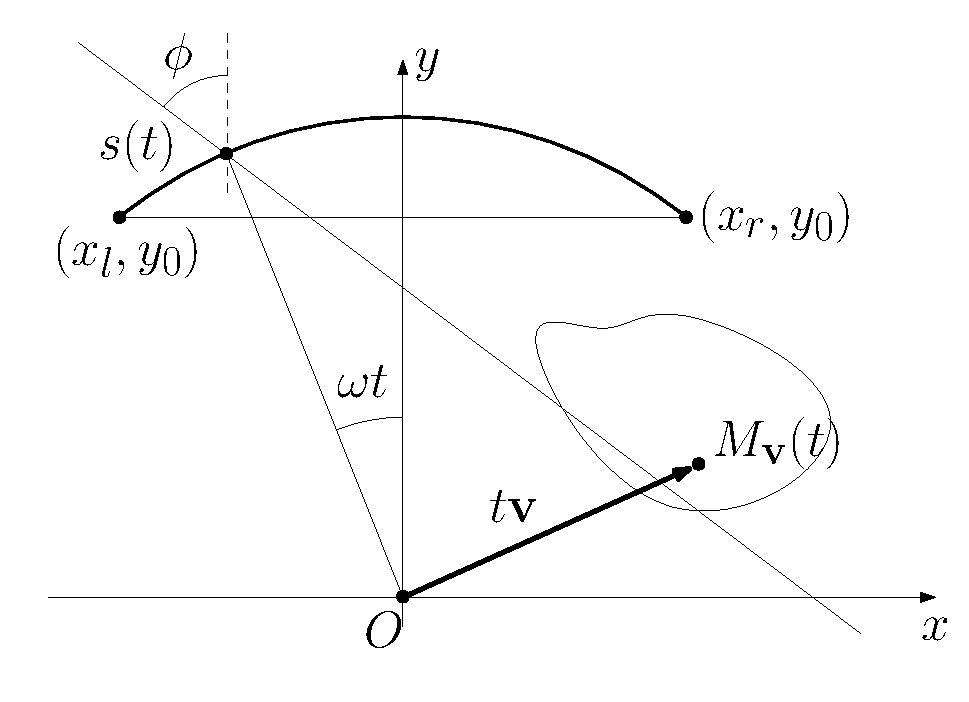
\includegraphics[width=75mm]{figs/frame_scanner.eps}
	\end{tabular}
	\caption{Problem under consideration. The source point $s(t)$ follows the arc of circle depicted in bold. The circle has center $O$ and radius $R_0$. The object is continually undergoing a translation during the movement of the source.\label{fig:notations}}
\end{figure}
The angular velocity of the source will be denoted $\omega$, and the time $t$ will range from $-T/2$ to $T/2$, where $T>0$. Hence, if we denote $s(t)$ the position of the source at time $t$, we have
\begin{equation}
	s(t) = \left( -R_0 \sin(\omega t), R_0 \cos(\omega t) \right).
\label{eq:source_position}
\end{equation}
Furthermore, we will let $s(T/2)=(x_l,y_l)$ (resp. $s(-T/2)=(x_r,y_r)$) denote the extreme left (resp. right) position of the source. Since $y_l = y_r = R_0 \cos(\omega T/2)$, we will call $y_0$ this common value. In the following, we will suppose that $\supp(\mu)$ lies in the half-space $\{ y < y_0 \}$, and that $y_0 > 0$ (\ie $0 < \omega T < \pi$).

We will suppose that at any time $t$ rays are simultaneously emitted from the source $s(t)$ with angle $\phi$ ranging from $-\pi/2$ to $\pi/2$. With this setup in mind, we can define the operator modeling the acquired data from the object.
\begin{definition}
The \emph{fanbeam projection data} of an object with density function $\mu$ is a function $(t,\phi) \mapsto \mathcal{F}\mu(t,\phi)$ defined by
\begin{equation}
	(\mathcal{F}\mu)(t,\phi) = \int_0^{+\infty} \mu \left( s(t) + l \left[ \sin \phi, -\cos \phi \right] \right) dl,
\end{equation}
where $t \in \left[ -T/2, T/2\right]$, $\phi \in \left[ -\pi/2, \pi/2\right]$ and $s(t)$ is given by~(\ref{eq:source_position}). The operator $\mu \mapsto \mathcal{F}\mu$ is called the \emph{fanbeam projection operator}.
\end{definition}


Now let us suppose that the object is translating along a line with a constant velocity vector $\bv = (v_1, v_2)\in \R^2$ (see Figure~\ref{fig:notations}, bottom). In other words, if we let $\Mbv(t)$ denote its center of mass at any time $t$, we have
\begin{equation}
	\Mbv(t) =   \left( t + T/2 \right) \bv
\label{eq:center_of_mass}
\end{equation}
The density function of the object now depends on both the spatial variable $\bx \in \R^2$ and the time $t$. If we denote the time varying object by $\mubv$, we have
\begin{equation}
	\mubv(t,\bx) = \mu\left( \bx - \Mbv(t)\right).
\end{equation}
In this regard, the fanbeam projection data will be modified in the following way.
\begin{definition}
The \emph{fanbeam projection data of a translating object} with density function $\mu$ and  velocity vector $\bv$ is given by
\begin{equation}
	(\Tbv\mu)(t,\phi) =  ( \mathcal{F} \mubv ) (t,\phi).
\label{eq:def_Tv}
\end{equation}
\end{definition}

The aim of this note is to derive data consistency conditions (DCCs) from~(\ref{eq:def_Tv}), in order to retrieve the velocity vector $\bv$ from the knowledge of a single element of the range of $\Tbv$.

\subsection{Derivation of DCCs}

In order to derive DCCs, we will first change our reference frame, from $\left(O, x, y\right)$ to $\left(M(t), x', y'\right)$, so that the origin is the center of mass of the object at any time t and the line between the start point and the end point of the source is still parallel to the $x'$-axis (see Figure~\ref{fig:change_frame}). In other words, we are performing the following change of variables
\begin{equation}
	(x,y) \leftrightarrow (x',y') = \mathcal{R}_{\beta} \left( (x,y)-\Mbv(t) \right),
\end{equation}
where $\mathcal{R}_{\beta}$ rotation by $\beta$. The angle beta is depicted in Figure~\ref{fig:change_frame} (top) and is given by
\begin{equation}
	\beta = \arctan \left( \frac{T v_2}{2R_0 \sin(\omega T/2) + T v_1} \right).
\end{equation}
Note that in this equation, the denominator can be equal to zero. Such situation occurs in particular when $v_1 < 0$. We studied those particular cases, both in terms of physical meaning and numerical implications. For the sake of simplicity, we will assume in this abstract that $v_1$ is not too negative (\emph{e.g.} $v_1 > - 2 R_0 / T$) to ensure that the denominator is non-zero.

\begin{figure}[!ht]
	\centering
	%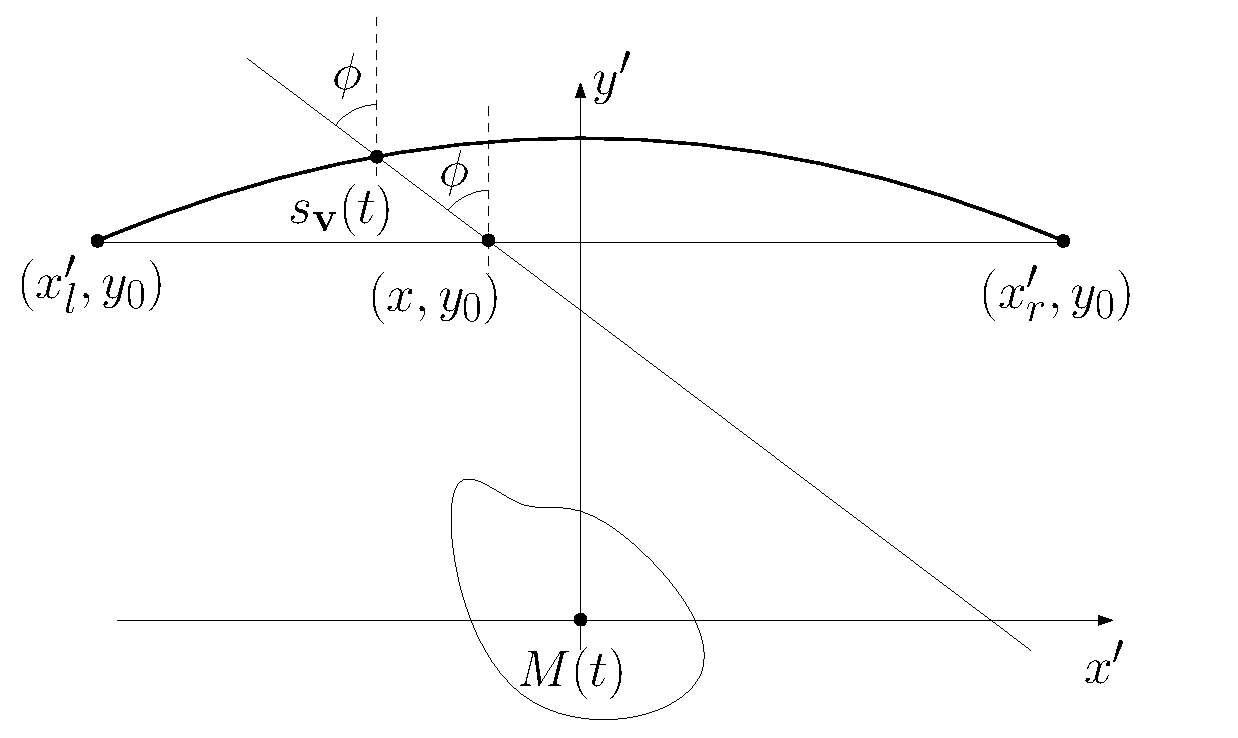
\includegraphics[width=12cm]{figs/frame_object.eps}
	\begin{tabular}{c}
	\includegraphics[width=75mm]{figs/frame_object_before_rotation.eps} \\
	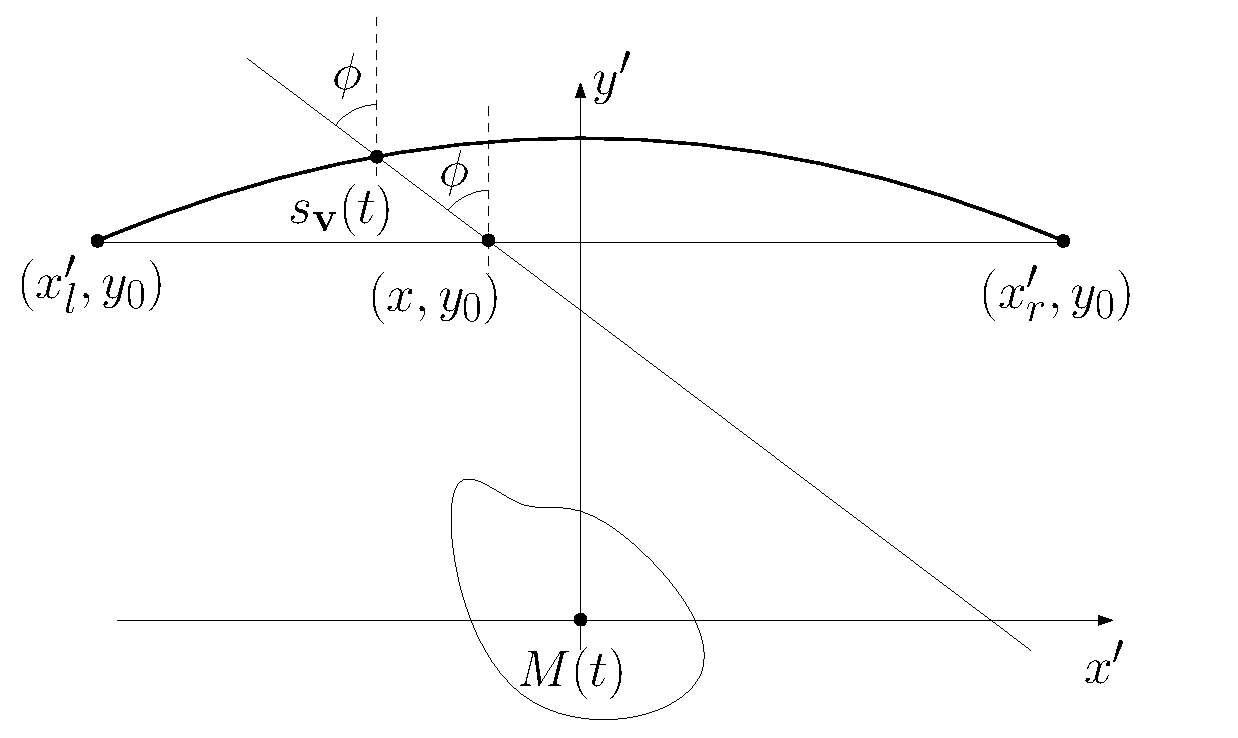
\includegraphics[width=75mm]{figs/frame_object.eps}
	\end{tabular}
	\caption{Change of frame: the object is now at center of the coordinates system. Top: only translation of the center of frame; bottom: after rotation of angle $\beta$. Note that the angle $\phi$ is the same as in Figure~\ref{fig:notations}, bottom. The virtual source position $(x',y_0')$ is defined in terms of $s_v(t)$ and $\phi$; see equation~(\ref{eq:x'}).\label{fig:change_frame}}
\end{figure}

In this frame, the coordinates of the source position is given by $\sbv(t)=\mathcal{R}_{\beta} \left( s(t)-\Mbv(t) \right)$. With this in mind, the data are given by the following formula
\begin{equation}
	(\Tbv\mu)(t,\phi) = \int_0^{+\infty} \mu \circ \mathcal{R}_{\beta} \left( s_{\bv}(t) + l \left[ \sin \phi, -\cos \phi \right] \right) dl.
\label{eq:F_from_sv}
\end{equation}

In other words, we are now dealing with a fixed object whose density function is given by $\mu \circ \mathcal{R}_{\beta}$ illuminated by a source following an arc of a cycloid in the frame $\left(M(t), x', y'\right)$ (see Figure~\ref{fig:change_frame}, bottom).

Here, the extreme points $\sbv(-T/2)$ and $\sbv(T/2)$ have the same $y'$-coordinate, $y'_0$. We will call $x'_l$ (resp. $x'_r$) the $x'$-coordinates of $\sbv(T/2)$ (resp. $\sbv(-T/2)$).

Now we define what we call the \emph{virtual fanbeam projection} from a point $(x',y'_0)$.
\begin{definition}
	For any point $x'$ between $x'_l$ and $x'_r$, and for any angle $\phi \in \left[ -\pi/2, \pi/2\right]$, the \emph{virtual fanbeam projection} of the object $\mu$ is defined by
\begin{equation}
	\left( \tilde{\mathcal{F}}\mu	\right)(x',\phi) = \int_0^{+\infty} \mu \left( (x',y'_0) + l \left[ \sin \phi, -\cos \phi \right] \right) dl.
\label{eq:def_Ftilde}
\end{equation}
This is called \emph{virtual} since it does not correspond to an actual position of the source.
\end{definition}

In the following lemma, we will make the connection between the virtual fanbeam projection and the fanbeam projection of the translating object.
\begin{lemma}
	Let us fix a time $t \in \left[ -T/2, T/2\right]$ and an angle $\phi \in \left[ -\pi/2, \pi/2\right]$. Let us define
	\begin{equation}
		x' = s_{1,\bv}(t) + \tan \phi \left( s_{2,\bv}(t) - y'_0 \right),
		\label{eq:x'}
	\end{equation}
	where, for any time $t$, $\left( s_{1,\bv}(t), s_{2,\bv}(t) \right)$ are the coordinates of $\sbv(t)$.
	Then, we have
	\begin{equation}
		\left( \tilde{\mathcal{F}}\mu \right)(x',\phi) = \left( \Tbv \mu \right)(t,\phi).
	\end{equation}
\label{lem:T_x_t}
\end{lemma}
The idea of the proof is to remark that between $x'$ and $\sbv(t)$, the integral of $\mu$ is equal to zero since the support is supposed to remain in the half-space $\left\{ y<y_0 \right\}$. Hence, instead of starting the integration from $x'$ in~(\ref{eq:def_Ftilde}), we can start from $\sbv(t)$, which will give us~(\ref{eq:F_from_sv})

We can now define what are the DCCs of our problem.
\begin{theorem}
\label{theo:main}
Let us fix a density function $\mu$. For any integer $n$, there exist a function $(x',t)\mapsto W_{n,v}(t,x') \in \Cinf \left( [-T/2,T/2] \times [x'_l,x'_r] \right)$ such that the function $B_n$ defined by
\begin{equation}
	B_n := x' \mapsto \int_{-T/2}^{T/2} \left( \Tbv \mu \right)\left( t,\lambda(t) \right) W_n(x',t,v) dt,
\label{eq:DCC}
\end{equation}
is a polynom of order $n$. In the formula above, the angle $\lambda(t)$ is defined by
\begin{equation}
	\lambda(t) = \arctan \left( F(x',t,\bv) \right),
\label{eq:def_lambda}
\end{equation}
where $F(x',t,\bv)$ is defined as a fraction $A/B$ with
\begin{dmath}
	A = x' + \cos \beta \left( R_0 \sin(\omega t) + \left( t + \frac{T}{2} \right)v_1 \right) + \\
	\sin \beta \left( R_0 \cos(\omega t) - \left( t + \frac{T}{2} \right)v_2 \right)
\end{dmath}
and
\begin{dmath}
	B = \cos \beta \left( R_0 \cos(\omega t) - \left( t + \frac{T}{2} \right)v_2 \right) - \sin \beta \left( R_0 \sin(\omega t) + \left( t + \frac{T}{2} \right)v_1 \right) - y'_0 
\end{dmath}
Moreover, it is possible to derive $W_{n,v}(t,x')$ analytically using the following formula
\begin{equation}
	W_{n,v}(t,x') = \tan^n F(x',t,\bv) \cos F(x',t,\bv) \frac{\partial F}{\partial t} (x',t,\bv)
\end{equation}
\end{theorem}

Here, the idea is to change variables in the following formula, which is known to be a polynom from~\cite{clackdoyle2013necessary}
\begin{equation}
	\int_{\pi/2}^{-\pi/2} \tilde{\mathcal{F}}\mu (x',\phi) \frac{\tan^n \phi}{\cos \phi} d\phi.
\label{eq:DCC_rolf}
\end{equation}
The change of variable occurs between $\phi$ in~(\ref{eq:DCC_rolf}) and $t$ in~(\ref{eq:DCC}) by using the definition in~\ref{eq:def_lambda}. This explains why the formulas in Theorem~\ref{theo:main}.

Although the formula giving $W_{n,v}(t,x')$ is quite heavy, we can observe that in the case $v_1=v_2=0$, we obtain the formula (7) in~\cite{clackdoyle2015consistency} since
\begin{equation}
	F \left( x',t,\bv = (0,0) \right) = \frac{x' + R_0 \sin(\omega t)}{R_0 \cos(\omega t)}
\end{equation}

\section{Numerical simulations}

\subsection{Principles}
\label{sub:principles}
Let us suppose that we have the projections $\left( \Tbv \mu \right)(t,\phi)$. In order to recover $v$, we can perform the following optimization procedure. Since $B_n(x')$ in equation~(\ref{eq:DCC}) is supposed to be a polynom of order $\leq n$, one can minimize
\begin{equation}
	\mathcal{J}(v) = \Vert \textrm{res} \left( B_n(\cdot,v) \right) \Vert^2
\label{eq:Jv}
\end{equation}
with respect to $v$, where $\textrm{res}$ is the residual of the projection onto $\R_n[X]$, and $n$ is the polynom degree to be taken into account. This will give us the velocity $v$ using only the knowledge of the data $\left( \Tbv \mu \right)(t,\phi)$.

\subsection{Application}
\label{sub:application}
Here, we will consider an object translating along the $x$-axis, \ie $v_2=0$. Indeed, we started with this particular case before tackling the more general one with $v_2 \neq 0$. Work is in progress and we hope to have the results for the CT-meeting conference. 

The object under consideration is an ellipse of uniform density, whose axis are $30$ and $15$ millimeters respectively, and making and angle of $45^{\circ}$ with respect to the $x$-axis. The source is rotating around the object with radius $R_0 = 600 \, \textrm{mm}$, with angle velocity $\omega = 1 \, \textrm{rad} \cdot \textrm{s}^{-1}$. The detector is a plane situated at a distance of $600 \, \textrm{mm}$ from the origin. The computations of the forward problem are performed using \verb+simpleRTK+, a Python's wrapping of \verb+RTK+~\cite{RTK}.

With a velocity of the ellipse given by $v_1 = 0.3 \textrm{mm} \cdot \textrm{s}^{-1}$, we obtain the sinogram depicted in Figure~\ref{fig:sinogram}.
\begin{figure}[!ht]
	\centering
	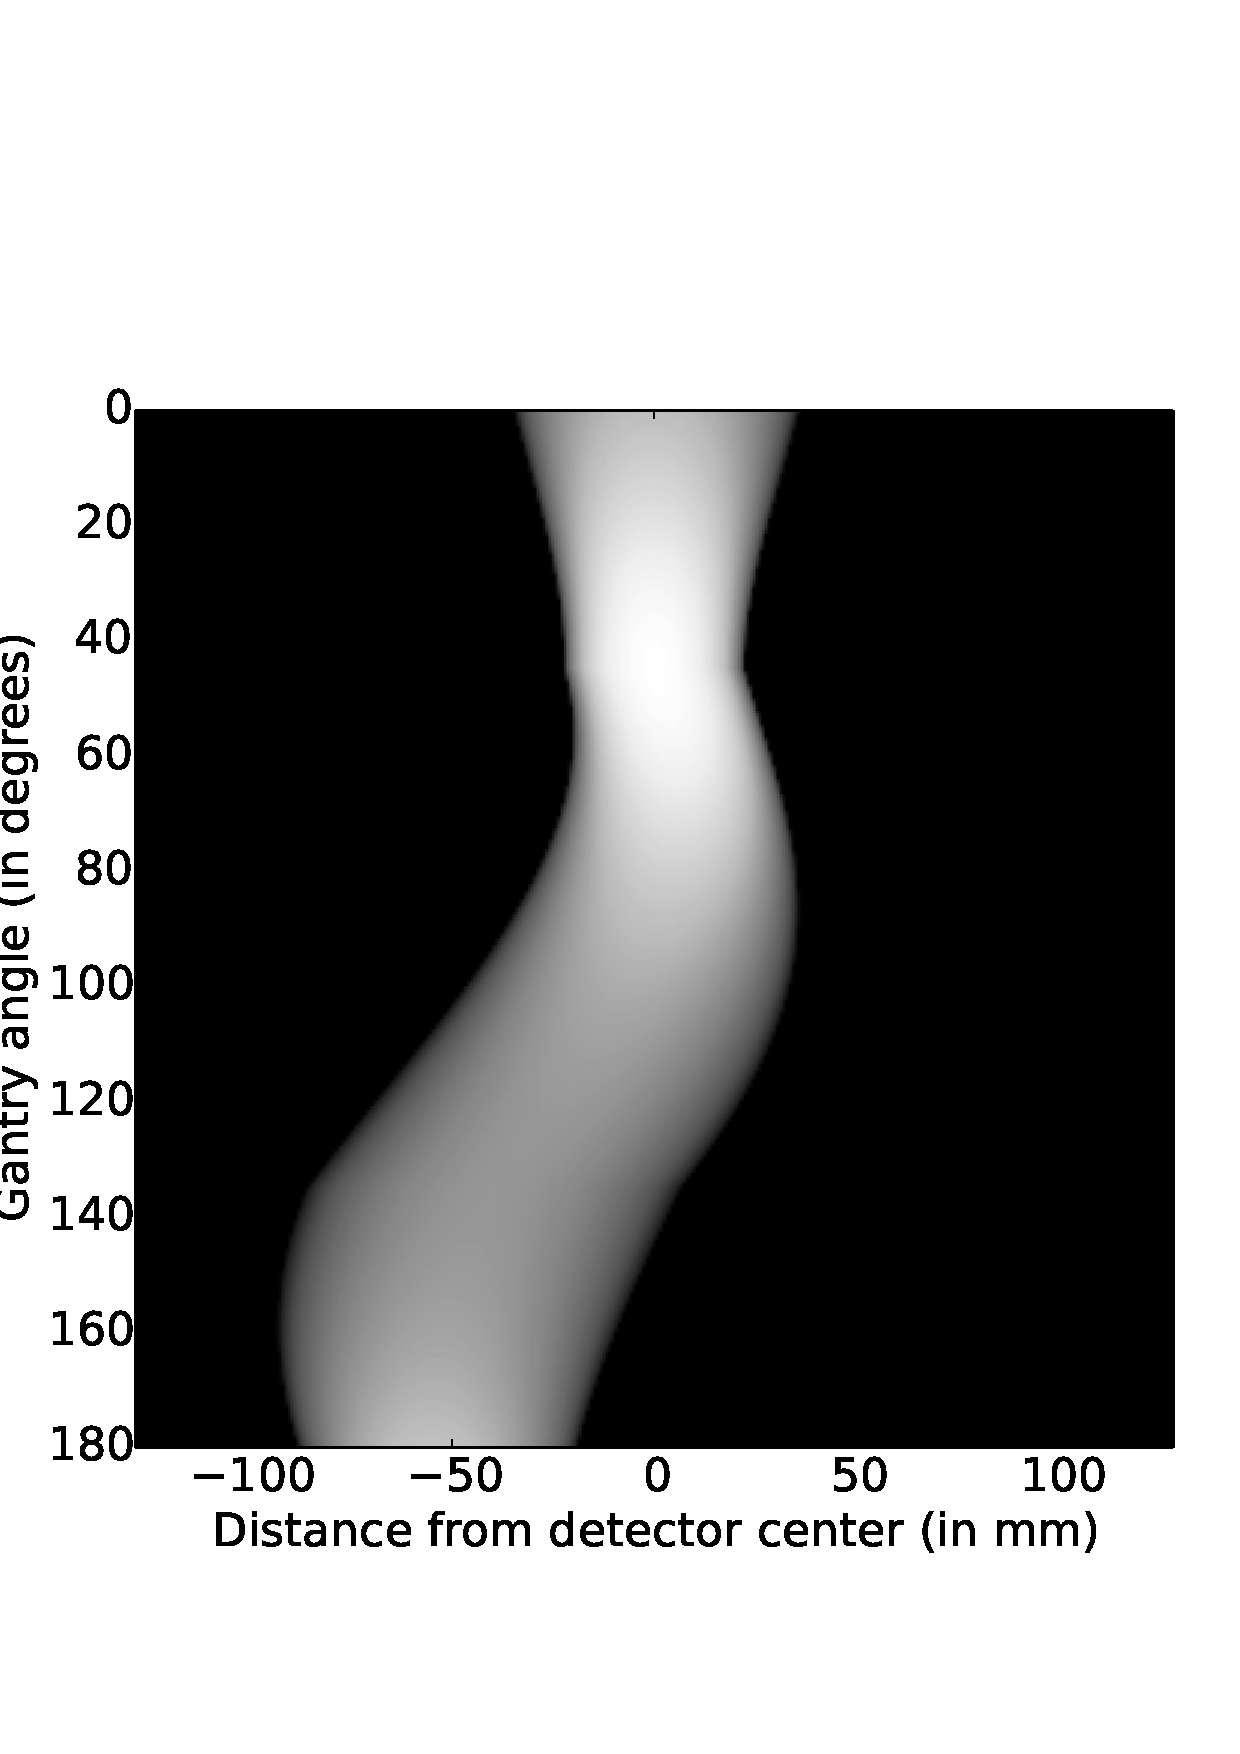
\includegraphics[width=75mm]{figs/sinogram.png}
	\caption{Sinogram of a moving ellipse, with semi-axis $a = 30$ and $b = 15$, translating along the $x$-axis with velocity $v_1 = 0.3$. It is illuminated by a source at distance $R_0 = 600$, rotating with angle velocity $\omega = 1$.\label{fig:sinogram}}
\end{figure}

With this configuration in mind, the functions $x' \mapsto B_n(x')$ for $n = 0,1,2,3$ can be visualized in Figure~\ref{fig:Bnx}. Note that the polynomial approximations are rather accurate. This can be seen by the fact that root mean square errors (RMSEs) between the actual values of $B_n(x)$ and their best polynomial approximations are low.
\begin{figure}
	\centering
	\begin{tabular}{cc}
	\includegraphics[width=75mm]{figs/B0.png} \\
	\includegraphics[width=75mm]{figs/B1.png} \\
	\includegraphics[width=75mm]{figs/B2.png} \\
	\includegraphics[width=75mm]{figs/B3.png} 
	\end{tabular}
	\caption{From top to bottom, functions $x' \mapsto B_n(x')$ for $n = 0,1,2,3$ respectively. Blue points are the actual data, while red lines are the best polynomial approximations. RMSE stands for root mean square error. The $x$-axis are expressed in millimeters.\label{fig:Bnx}}
\end{figure}

With this velocity $v_1 = 0.3$, and with a degree of polynom $n = 2$, we performed the minimization of the functionnal $\mathcal{J}(v)$ defined in~(\ref{eq:Jv}). For this purpose, we used Powell's conjugate direction method~\cite{powell1964efficient}, which does not require differentiation of the functionnal. We studied the influence of the time during which the object is translating, see Table~\ref{tab:results} for full results, where $\hat{v}$ stands for the estimated value for the velocity $v_1$.. We can observe that there is a limit below which the accuracy decrease dramatically. Further investigations are in progress, where the influence of all other parameters are studied.

\begin{table}[!ht]
\caption{Results of optimization \label{tab:results}}
\centering
	\begin{tabular}{c|c|c}
	  $T$ & $\hat{v}$ & $\Vert v_1 - \hat{v}\Vert$ \\
	  \hline
		$95$ & $0.30$0 & $5.55 \cdot 10^{-17}$ \\
		$90$ & $0.300$ & $1.11 \cdot 10^{-16}$ \\
		$85$ & $0.300$ & $1.11 \cdot 10^{-16}$ \\
		$84$ & $0.300$ & $0$ \\
		$83$ & $0.300$ & $0$ \\
		$82$ & $0.376$ & $7.60 \cdot 10^{-2}$ \\
		$81$ & $0.415$ & $0.115$ \\
		$80$ & $0.436$ & $0.136$ \\
		$75$ & $0.436$ & $0.136$
\end{tabular}
\end{table}


\section{Conclusion}
In this work, we have proposed a way to recover the velocity parameters of a translating object in fanbeam CT from a set of projections restricted to an arc of the circular trajectory. The method uses the so-called data consistency conditions (DCCs), adapted from~\cite{clackdoyle2015consistency}. Setting the origin of the frame in the center of mass of the object, we are in fact dealing with DCCs in the case of an arc of a cycloid. Numerical examples show that these conditions work well in the case of an object translating in a direction which is parallel to the $x$-axis. Further work is under progress to recover the same results in the general translation.


\bibliographystyle{plain}
\bibliography{DCC_translation}


\end{document}

